\newif\ifarxiv
\arxivtrue % comment out for BMVC

\ifarxiv
    \documentclass{article}
    \usepackage[margin=1.2in]{geometry}
    \makeatletter
    \newcommand\footnoteref[1]{\protected@xdef\@thefnmark{\ref{#1}}\@footnotemark}
    \makeatother
\else
  \documentclass{bmvc/bmvc2k}
  %% Enter your paper number here for the review copy
  % \bmvcreviewcopy{965}
\fi

% \documentclass{article}

% spacing for editting -------
%\usepackage{setspace}
%\doublespacing
%\onehalfspacing
% spacing for editting -------

% my packages {
%\usepackage{times}
% not sure if these are allowed in CVPR:
\usepackage{bm}
\usepackage{enumitem}
% Definitions of handy macros can go here
%\usepackage{epsfig}
%\usepackage{amsmath}
%\usepackage{amssymb}
%\newcommand{\dataset}{{\cal D}}
%\newcommand{\fracpartial}[2]{\frac{\partial #1}{\partial  #2}}
% Include other packages here, before hyperref.
%\usepackage[breaklinks=true,bookmarks=false]{hyperref}
\usepackage{siunitx}
\usepackage{tikz}
\usetikzlibrary{calc,arrows.meta,positioning,decorations.markings}
\usepackage{amsfonts}
\usepackage{amsmath}

\usepackage[linesnumbered,ruled]{algorithm2e}
%\usepackage[linesnumbered,ruled,vlined]{algorithm2e}
\newcommand\mycommfont[1]{\footnotesize\ttfamily\textcolor{gray}{#1}}
\SetCommentSty{mycommfont}

%\usepackage{siunitx}
%\usepackage{dcolumn,booktabs}
%\newcolumntype{d}[1]{D{.}{.}{#1}}
%\newcommand\mc[1]{\multicolumn{1}{c}{#1}} % handy shortcut macro
%\usepackage[none]{hyphenat} % Inserted this to not have line splits  -'s
%\usepackage{enumitem}
%\usepackage{subcaption}
%\usepackage{gensymb}
%\usepackage{stmaryrd}
%\usepackage{fancyhdr}
%\usepackage{relsize}
% } my packages

% Recommended, but optional, packages for figures and better typesetting:
\usepackage{microtype}
\usepackage{graphicx,calc}
\usepackage{subfigure}
\usepackage{booktabs} % for professional tables

% hyperref makes hyperlinks in the resulting PDF.
% If your build breaks (sometimes temporarily if a hyperlink spans a page)
% please comment out the following usepackage line and replace
% \usepackage{icml2018} with \usepackage[nohyperref]{icml2018} above.
\usepackage{hyperref}

%\usepackage[percent]{overpic}

% Attempt to make hyperref and algorithmic work together better:
\newcommand{\theHalgorithm}{\arabic{algorithm}}

\newlength\myheight
\newlength\mydepth
\settototalheight\myheight{Xygp}
\settodepth\mydepth{Xygp}
\setlength\fboxsep{0pt}
\newcommand*\inlinegraphics[1]{%
  \settototalheight\myheight{Xygp}%
  \settodepth\mydepth{Xygp}%
  \raisebox{-\mydepth}{\includegraphics[height=\myheight]{#1}}%
}

\renewcommand*\ttdefault{lcmtt}
\newcommand\ndash{\mathop{\mbox{$n$-}}}
\newcommand\dashw{\mathop{\mbox{-$\mathsf{w}$}}}
%\newcommand{\TMS}{{\mkern-2mu\times\mkern-2mu}}
\newcommand{\TMS}{{\mkern-1.5mu\times\mkern-1.5mu}}

\newenvironment{tightitemize}
{ \begin{itemize}
    \setlength{\itemsep}{4pt}
    \setlength{\parskip}{0pt}
    \setlength{\parsep}{0pt}     }
{ \end{itemize}                  }

\usepackage{mathtools}
\DeclarePairedDelimiter\ceil{\lceil}{\rceil}
\DeclarePairedDelimiter\floor{\lfloor}{\rfloor}

% Use the following line for the initial blind version submitted for review:
%\usepackage{icml/icml2018}

% If accepted, instead use the following line for the camera-ready submission:
% \usepackage[accepted]{icml/icml2018}

% The \icmltitle you define below is probably too long as a header.
% Therefore, a short form for the running title is supplied here:
% \icmltitlerunning{Knowledge and Techniques Matter}

\begin{document}

%\raggedbottom

\ifarxiv
	\title{A New Benchmark and Progress Toward Improved Weakly Supervised Learning}
	\author{Jason Ramapuram\footnote{Equal contributions.}
          \footnote{University of Geneva \& University of Applied
            Sciences, Western
          Switzerland}\ , jason@ramapuram.net \\ Russ Webb\textsuperscript{*}\footnote{Apple Inc, Cupertino, CA}\ , rwebb@apple.com}
	\maketitle
\else
        % \twocolumn[
        %\icmltitle{Knowledge and Techniques Matter: \\Exploring the Limits of Weakly Supervised Learning}
        %\title{All-Pairs: Benchmarking the Limits of Weakly Supervised Learning}
        %\title{Learned Spatial Histograms and Benchmarking Weakly Supervised Learning}
        %\title{Learned Spatial Histograms to Improve a Benchmarks of Weakly Supervised Learning}
        %\title{Learned Spatial Histograms to Improve Weakly Supervised Learning}
        % A New Benchmark and Improvements for Weakly Supervised Learning
        \title{A New Benchmark and Progress Toward Improved Weakly Supervised Learning}
        % All-Pairs: A Benchmark for Weakly Supervised Learning
        \addauthor{Jason Ramapuram}{jason@ramapuram.net}{2}
        \addauthor{Russ Webb}{rwebb@apple.com}{1}

        % Enter the institutions
        % \addinstitution{Name\\Address}
        \addinstitution{
          Apple Inc\\
          Cupertino, California, USA
        }
        \addinstitution{
          University of Geneva \& \\University of Applied Sciences, \\
          Western Switzerland
        }

        \runninghead{Ramapuram, Webb}{Toward Improved Weakly Supervised Learning}

        % \vskip 0.3in
        % ]
        \maketitle
\fi


% this must go after the closing bracket ] following \twocolumn[ ...

% This command actually creates the footnote in the first column
% listing the affiliations and the copyright notice.
% The command takes one argument, which is text to display at the start of the footnote.
% The \icmlEqualContribution command is standard text for equal contribution.
% Remove it (just {}) if you do not need this facility.

%\printAffiliationsAndNotice{}  % leave blank if no need to mention equal contribution
% \printAffiliationsAndNotice{\icmlEqualContribution} % otherwise use the standard text.

% =========================================================

\begin{abstract}%   <- trailing '%' for backward compatibility of .sty file
{\em Knowledge Matters: Importance of Prior Information for Optimization} \cite{gulccehre2016knowledge}, by G\"{u}l\c{c}ehre et. al.,
sought to establish the limits of current black-box, deep learning
techniques by posing problems which are difficult to learn without engineering
knowledge into the model or training procedure.  In our work, we
solve the previous {\em Knowledge Matters} problem with 100\% accuracy
using a generic model, pose a more
difficult and scalable problem, All-Pairs, and advance this new problem
by introducing a new learned, spatially-varying histogram model called TypeNet which outperforms conventional
models on the problem.  We present results on All-Pairs where our model
achieves 100\% test accuracy while the best ResNet models achieve 79\%
accuracy.  In addition, our model is more than an order of magnitude smaller than Resnet-34.  The challenge of solving larger-scale
All-Pairs problems with high accuracy is presented to the community for investigation.
\end{abstract}

\section{Introduction}

Scientific literature is most commonly available in the form of PDFs, which pose challenges for accessibility \citep{NielsenPDFStillUnfit, Bigham2016AnUT}. When researchers, students, and other individuals who are blind or low vision (BLV) interact with scientific PDFs through screen readers, the availability of document structure tags, labeled reading order, labeled headers, and image alt-text are necessary to facilitate these interactions. However, these features must be painstakingly added by authors using proprietary software tools, and as a result, are often missing from papers. Low vision or dyslexic readers who interact with PDFs through screen magnification or text-to-speech may also find the complexity of certain academic paper PDF formats challenging, e.g., non-linear layout can interrupt the flow of text in a magnifying tool. Inaccessible paper PDFs can lead to high cognitive overload, frustration, and abandonment of reading for BLV readers. 

Unfortunately, we find that the majority of scientific PDFs lack basic accessibility features. We estimate based on a sample of \numpdfs PDFs from multiple fields of study that only around \percaccessible of paper PDFs released in the last decade satisfy all of the aforementioned accessibility requirements. 
Accessibility challenges for academic PDFs are largely due to three factors: (1) the complexity of the PDF file format, which make it less amenable to certain accessibility features, (2) the dearth of tools, especially non-proprietary tools, for creating accessible PDFs, and (3) the dependency on volunteerism from the community with minimal support or enforcement \citep{Bigham2016AnUT}. The intent of the PDF file format is to support faithful visual representation of a document for printing, a goal that is inherently divergent from that of document representation for the purposes of accessibility. Though some professional organizations like the Association for Computing Machinery (ACM) have encouraged PDF accessibility through standards and writing guidelines,\footnote{\href{https://www.acm.org/publications/authors/submissions}{https://www.acm.org/publications/authors/submissions}} uptake among academic publishers and disciplines more broadly has been limited. 

While policy changes help, the fact remains that most academic PDFs produced today, and historically, are inaccessible, yet remain as the dominant way to read those papers. A long-range solution will necessitate buy-in from multiple stakeholders---publishers, authors, readers, technologists, granting agencies, and the like. But in the interim, there are technological solutions that can be offered as a sort of ``band-aid'' to the problem. We use this paper to offer an in-depth qualitative and quantitative description of the problem as it stands, and to introduce one such technological solution: the \scially system that automatically extracts semantic information from paper PDFs and re-renders this content in the form of an accessible HTML document. Though the process is imperfect and can introduce errors, we demonstrate the ability of the rendered HTMLs to reduce cognitive load and facilitate in-paper navigation and interactions for BLV users. 

The goals and contributions of this paper are three-fold:

\begin{enumerate}
    \item We characterize the state of academic-paper PDF accessibility by estimating the degree of adherence to accessibility criteria for papers published in the last decade (2010--2019), and describe correlations between year, field of study, PDF typesetting software, and PDF accessibility.
    \item We propose an automated approach for extracting the content of academic PDFs and displaying this content in a more accessible HTML document format. We build a prototype that re-renders 12 million PDFs in HTML, and describe the design decisions, features, and quality of the renders (assessed as faithfulness to the source PDF). We perform expert grading of the rendered HTML and report an error analysis. A demo of our system is available at \href{https://scia11y.org/}{scia11y.org}, which makes available 1.5M HTML renders of open access PDFs.
    \item We conduct an exploratory user study with \numusers BLV scholars to better understand the challenges they experience when reading academic papers and how our proposed tool might augment their current workflow. During the study, we ask users to interact with the prototype and offer feedback for its improvement. We perform open coding of interviews to identify existing reading challenges, coping mechanisms, as well as positive and negative responses to prototype features. We summarize the findings of this user study into a set of design recommendations.
\end{enumerate}

Our analysis reveals that PDF accessibility adherence is low across all fields of study. Of the five accessibility criteria we assess, only \percaccessible of the PDFs we assess demonstrate full compliance. Though compliance for several criteria seems to be increasing over time, author awareness and contribution to accessibility remains low, as Alt-text has the lowest compliance of the five criteria at between 5--10\% (Alt-text is the only criterion of the five that \textit{requires} author intervention in all cases using current tools). We also find that typesetting software is strongly associated with accessibility compliance, with LaTeX and publishing software like Arbortext APP producing low compliance PDFs, while Microsoft Word is generally associated with higher compliance.


\begin{figure}[t!]
    \centering
    \includegraphics[width=\textwidth]{figures/pipeline.png}
    \caption{A schematic for creating the \scially HTML render from a paper PDF. Starting with the raw two-column PDF on the left, S2ORC \citep{lo-wang-2020-s2orc} is used to extract title, authors, abstract, section headers, body text, and references. S2ORC also identifies links between inline citations and references to figures and table objects. DeepFigures \citep{Siegel2018ExtractingSF} is used to extract figures and tables, along with their captions. The output of these two models are merged with metadata from the Semantic Scholar API. Heuristics are used to construct a table of contents, to insert figures and tables in the appropriate places in the text, and to repair broken URLs. We add HTML headers as illustrated (header tags for sections, paragraph tags for body text, and figure tags for figures and tables); highlighted components (table of contents and links in references) are not in the PDF and novel navigational features that we introduce to the HTML render. An example HTML render of parts of a paper document is show to the right (actual render is single column, which is split here for presentation).}
    \label{fig:pipeline}
    \Description{A schematic diagram showing the components of the SciA11y pipeline. An image of a paper PDF is on the left. Red boxes on the PDF image highlight the text components from the paper, with an arrow pointing to a box that says "S2ORC extracts: title, authors, abstract, section headers, body paragraphs, and references." A blue box on the PDF image highlights a figure, with an arrow pointing to a box that says "DeepFigures extracts: figures, figure captions, tables, and table titles/captions." A box below "S2ORC extracts" and "DeepFigures extracts" says "Additional content: metadata from Semantic Scholar API, table of contents, figures and tables inserted at first mention, and links between references and text." Arrows from all three boxes point into a larger box that describes the SciA11y prototype, where HTML tags are inserted around various blocks of text extracted from the PDF. On the right of all this is a screen capture of an example HTML render, showing how the semantic content from the PDF is represented as a single-column HTML page for easy reading.}
\end{figure}

To offset the reading challenges of inaccessible papers for BLV researchers, we propose and test the \scially system for rendering academic PDFs into accessible HTML documents. As shown in Figure~\ref{fig:pipeline}, our prototype integrates several machine learning text and vision models to extract the structure and semantic content of papers. The content is represented as an HTML document with headings and links for navigation, figures and tables, as well as other novel features to assist in document structure understanding. Our evaluation of the \scially system identifies common classes of extraction problems, and finds that though many papers exhibit some extraction errors, the majority (55\%) have no major problems that impact readability, and another 32\% have only some problems that impact readability.

Through our user study, we identify numerous challenges faced by BLV users when reading paper PDFs, including some that affect the whole document or limit navigation, and many that affect the ability of the reader to understand text or various elements of a paper like math content or tables. Responses to \scially were positive; participants especially liked navigation features such as headings, the table of contents, and bidirectional links between inline citations and references. Of the extraction errors in \scially, missed or incorrectly extracted headings were the most problematic, as these impact the user's ability to navigate between sections and fully trust the system. All users reported being likely to use the system in the future. When asked how the system might be integrated into their workflow, one participant replied ``I think it would become the workflow.'' Another participant said, ``for unaccessible PDFs, this is life-changing.'' We condense these findings into a set of recommendations for designing and engineering accessible reading systems (Section~\ref{sec:designrecs}). Most importantly, documents should be structured to match a reader's mental model, objects should be properly tagged, and care should be taken to reduce the reader's cognitive load and increase trust in the system. Features that emulate the external memory that visual layout provides to sighted users can be especially beneficial.

This paper is organized as follows. Following a description of related work in Section \ref{sec:related_work}, we first provide a meta-scientific analysis of the current state of academic PDF accessibility in Section \ref{sec:sos}. In Section \ref{sec:pdf2html}, we document our pipeline for converting PDF to HTML and describe the \scially prototype for rendering papers. An evaluation of HTML render quality and faithfulness is provided in Section \ref{sec:evaluation}. Section \ref{sec:user_study} describes our user study and findings. 
We recognize that no PDF extraction system is perfect, and many open research challenges remain in improving these systems. However, based on our findings, we believe \scially can dramatically improve screen reader navigation of most papers compared to PDFs, and is well-positioned to assist BLV researchers with many of their most common reading use cases. Our hope is that a system such as \scially can improve BLV researcher access to the content of academic papers, and that these design recommendations can be leveraged by others to create better, more faithful, and ultimately more usable tools and systems for scholars in the BLV community.

\section{Related Work}
\label{sec:related_work}
% In this section, we review the related work, which includes graph neural networks, and robust graph neural networks. 

\subsection{Graph Neural Networks}
Graph Neural Networks (GNNs) have shown their great power in modeling graph structured data for various applications~\cite{wang2019semi,wang2018cross,zhao2020semi,dai2021say,zhao2021graphsmote}.
To generalize neural networks for graphs, two categories of GNNs are proposed, i.e., spectral-based~\cite{bruna2013spectral,henaff2015deep,kipf2016semi,levie2018cayleynets} and spatial-based~\cite{velivckovic2017graph,hamilton2017inductive,chen2018fastgcn,chiang2019cluster}. \citeauthor{bruna2013spectral} \cite{bruna2013spectral} first propose spectral-based GNNs by defining graph convolution with spectral graph theory. For instance, GCN~\cite{kipf2016semi} simplifies the convolutional operation by using the first order approximation. Spatial-based graph convolution is defined in spatial domain, which updates node representation by aggregating its neighbors' representations \cite{niepert2016learning,gilmer2017neural,hamilton2017inductive}. 
For example, self-attention of neighbor nodes is leveraged in graph attention network (GAT) \cite{velivckovic2017graph}. Moreover, various spatial methods are proposed to solve the scalability issue~\cite{chen2018fastgcn,chiang2019cluster} and learn deeper GNNs~\cite{chen2020simple}.  Recently, to alleviate the problem of lacking labeled nodes, many efforts are taken to explore GNNs using self-supervision, which aims to learn better node representations with pretext tasks~\cite{sun2019multi,li2018deeper,kim2021find,zhu2020self,jin2020self,dai2021towards}. For instance, superGAT~\cite{kim2021find} deploys edge prediction in GAT to guide the learning of attention for better representations. SE-GNN~\cite{dai2021towards} deploys contrastive learning to benefit the similarity modeling for self-explainable GNN.

Inspired by the great success of GNNs, methods that construct graphs and adopt GNNs for data without explicit relational structure are also explored~\cite{henaff2015deep,chen2019multi,jiang2019semi,dai2021nrgnn}. Generally, a graph would be built based on certain rules~\cite{henaff2015deep,chen2019multi} or be learned in an end-to-end model~\cite{jiang2019semi,dai2021nrgnn}. Our RS-GNN is inherently different from these methods as we eliminate/down-weight the noisy edges and predict the missing edges for robust GNNs on noisy graphs with limited labels. 

\subsection{Robust GNNs}
Although GNNs have obtained great achievements, they are vulnerable to adversarial attacks~\cite{wu2019adversarial,dai2018adversarial,zugner2018adversarial,zugner2019adversarial}. Based on the objective, the adversarial attacks on GNNs can be split into two categories, i.e., targeted attack~\cite{dai2018adversarial,zugner2018adversarial} and non-targeted attack~\cite{zugner2019adversarial}. Targeted attack methods aim to degrade the performance of the GNNs on target nodes. 
For instance, \textit{nettack}~\cite{zugner2018adversarial} adds adversarial perturbations to a graph to attack targeted nodes. Non-targeted attack aims to reduce the overall performance of GNNs. For example, \textit{metattack}~\cite{zugner2019adversarial} poisons the graph globally to achieve non-targeted attack with meta-learning. To defend against adversarial attacks, many efforts are taken recently~\cite{zhu2019robust,wu2019adversarial,entezari2020all,jin2020graph,tang2020transferring,zhang2020gnnguard}. \cite{wu2019adversarial} prune the perturbed edges based on Jaccard similarity of node features. Another preprocessing method by low-rank approximation of adjacent matrix is investigated~\cite{entezari2020all}. Pro-GNN~\cite{jin2020graph} is the most similar work to ours, which learns a clean graph structure by low-rank constraint. However, they only tackle the adversarial edges and their computational cost is very large due to the direct learning of the graph and the sparse low-rank constraint.
This work is inherently different from these methods as: (i) we study a novel problem of developing robust GNN for both noisy graphs and label sparsity issues; and (ii) the proposed RS-GNN simultaneously tackles the two issues by learning an link predictor to 
down-weight noisy edges and connecting nodes with high similarity to facilitate message-passing; 
and (iii) RS-GNN uses link predictor instead of direct graph learning to save computational cost. 
% ==================================================
\section{Solving the Pentomino Problem}
% -----------------------------------
% -----------------------------------

\begin{figure*}[!htb]
\minipage[t]{0.468\textwidth}
  \includegraphics[width=\linewidth]{images/pentomino}
  \endminipage\hfill
\minipage[t]{0.532\textwidth}
  \includegraphics[width=\linewidth]{images/km_solved.png}
\endminipage\hfill
\caption{\emph{Left}: The Pentomino sprites and two examples illustrating the $true$ and $false$ classes.
  \emph{Right}: Test accuracy (median and inner quartiles, 10 trials) on the Pentomino problem with and without modern training advances. Note, log-scale of x-axis.}
\label{pento_sprites}
\end{figure*}

{\em Knowledge Matters} \cite{gulccehre2016knowledge} explores the extent to
which neural networks are able to learn problems given minimal
supervised information. Their formulation has a fully defined loss
function; however, the gradient of the loss with respect to the
parameters provides no direct information about potentially useful
subtasks such as segmentation, object classification, or counting. They concluded that the networks and training methods they tested converged to a
local minima.

The {\em Knowledge Matters} demonstration utilized the Pentomino dataset, which
is formed from a set of sprites \cite{gulcehre_2015}
shown in Figure \ref{pento_sprites}. The
dataset is generated by placing three sprites onto a canvas $C \in
\mathbb{R}^{64\TMS64}$. Each sprite undergoes a random rotation 
(\ang{0}, \ang{90}, \ang{180}, or \ang{270}) and integer scaling ($1\times$ or $2\times$).  The goal of the
neural network is to predict a 1 if the rotated and scaled sprites in an
image are the same and 0 otherwise. One possible solution to the
Pentomino problem is to learn to segment, classify, and count the number
of underlying objects in the image. The challenge (claimed impossible in \cite{gulcehre_2015})
is to find a solution using a generic network given only the binary
label for each image.

G\"{u}l\c{c}ehre et. al \cite{gulccehre2016knowledge} observed that
``black-box machine  learning  algorithms  could  not  perform  better 
than  chance on [the Pentomino problem].'' Decomposing
the problem into two stages however, made the task easily solvable. The
first stage in the decomposition was a classification
step, where extra label information was provided to the model. Given the
predicted classes, the second stage projected this output to the Bernouili
log-likelihood objective. Using some of the recent advances in 
DNN training, we are able to completely solve the original
problem demonstrated in {\em Knowledge Matters}; we do so without the
requirement of an intermediary model or the addition of extra
information. We also experimented with a reproduction of the model 
proposed in the paper and found that given enough time (over 1000
epochs) the model does make progress on the Pentomino problem, as shown
in Figure \ref{pento_sprites} in gray. This observation is in line with
recent insights of \cite{hoffer2017train} that discuss the effects of
training duration and batch size.

The fully-connected (fc) model presented in \cite{gulccehre2016knowledge} was composed of layer sizes
[2050, 11, 1024] and trained with ADADelta \cite{zeiler2012adadelta} and weight regularization. The 11-unit layer
served as a bottleneck to bring structural information into the
network.  We leverage four recent advances to solve the Pentomino problem: Batch
Normalization (BN) \cite{ioffe2015batch}, Exponential Linear Units
\cite{clevert2015fast}, the Adam optimizer \cite{kingma2014adam}, and
Xavier initializations \cite{glorot2010understanding}. In constrast to
the large model employed in \cite{gulccehre2016knowledge}, we use a
fully-connected network with layer sizing of
$[32, 64, 12, 32, 8]$; this translates to a 98.5\% reduction of the
total number of model parameters. Comparable in size to the largest
training sets used in \cite{gulccehre2016knowledge}, 486k
samples were used for training and 54k samples were held out for testing.

G\"{u}l\c{c}ehre et. al \cite{gulccehre2016knowledge} were only able to
train black-box (generic), fully-connected models to achieve 50\% accuracy on the
Pentomino dataset. Their best model, after significant
hyper-parameter search, resulted in a 5.3\% training and 6.7\% test error
on the 80k Pentomino training dataset. This performance was achieved 
via a two-stage network that induced structural information
into the neural network. On the same training set, we achieved a 1\% error using a black-box neural network with the
5-layer network described above.  Figure
\ref{pento_sprites} shows the training accuracy for the original
{\em Knowledge Matters} network (gray), our modification (blue), and our TypeNet model (green, see Section \ref{typenetdetails}) on
the Pentomino problem (note the log scale on the x-axis).

%%% Local Variables:
%%% mode: latex
%%% TeX-master: "0.knowledge_and_techniques_matter"
%%% End:

% ==================================================
\section{The All-Pairs Problem} \label{all_pairs}
% -----------------------------------
\begin{figure}[h!]
\vskip 0.2in
\begin{center}
\scalebox{0.6}{\centerline{\includegraphics[width=\columnwidth]{images/all_pairs_survey}}}
\caption{All-Pairs examples from 2-2 on the left to 8-8 on the right.  The bottom row is $true$ and the top row is $false$.}
\label{example8}
\end{center}
\vskip -0.2in
\end{figure}


\subsection{Definition and Examples}

Extending the ideas in the Pentomino problem, we use anti-aliased white
symbols on a black background to construct the following new problem.
The \textit{N-K} All-Pairs problem contains \textit{2N} symbols from an
alphabet of \textit{K} choices.  Each example is \textit{true} if each of its
symbols pairs with a symbol of the same type without reuse,
and \textit{false} otherwise.  Symbols are positioned randomly with no
overlap.  Symbols are of similar scales, ranging from
10--18 pixels across, and have differing symmetries (for instance, some
are rotationally invariant, while others are not).  The exact structure
and variations of each symbol are given by the generator code supplied
online \cite{allpairs2018}.

Each symbol is shown below with the
number of unique ways it can appear, as configured in our experiments.  In contrast, the
Pentomino problem used 8
variations for each symbol. The symbols are used in the order given, so the 4-4 All-Pairs problem will use \textbf{circle}, \textbf{line}, \textbf{cross}, and \textbf{angle}.  For this work a $76\TMS76$ image is used for $N<6$ and a
$96\TMS96$ image is used for larger $N$.

\begin{table}[htp]
  \begin{center}
\scalebox{0.9}{
\begin{tabular}{r r l r r r l r}
id & name & examples & cardinality &id & name & examples & cardinality \\
\hline
1 & \textbf{circle}        & \inlinegraphics{images/strip_0.png}  & 165   & 10 & \textbf{box}          & \inlinegraphics{images/strip_9.png}  & 480   \\
2 & \textbf{line}          & \inlinegraphics{images/strip_1.png}  & 174   & 11 & \textbf{box-diagonal} & \inlinegraphics{images/strip_10.png} & 518   \\
3 & \textbf{cross}         & \inlinegraphics{images/strip_2.png}  & 45.3k & 12 & \textbf{barbell}      & \inlinegraphics{images/strip_11.png} & 78    \\
4 & \textbf{angle}         & \inlinegraphics{images/strip_3.png}  & 39k   & 13 & \textbf{dot-line}     & \inlinegraphics{images/strip_12.png} & 156   \\
5 & \textbf{3-star}        & \inlinegraphics{images/strip_4.png}  & 1.43M & 14 & \textbf{z}            & \inlinegraphics{images/strip_13.png} & 518   \\
6 & \textbf{theta}         & \inlinegraphics{images/strip_5.png}  & 20k   & 15 & \textbf{triangle-lid} & \inlinegraphics{images/strip_14.png} & 1036  \\
7 & \textbf{phi}           & \inlinegraphics{images/strip_6.png}  & 20k   & 16 & \textbf{dot-mid-line} & \inlinegraphics{images/strip_15.png} & 78    \\
8 & \textbf{2-circle}      & \inlinegraphics{images/strip_7.png}  & 7k& 17 & \textbf{hourglass}    & \inlinegraphics{images/strip_16.png} & 518   \\
9 & \textbf{circle-3star}  & \inlinegraphics{images/strip_8.png}  & 7.15M& 18 & \textbf{triangle}     & \inlinegraphics{images/strip_17.png} & 11.8k \\
\end{tabular}
}
\end{center}
\label{default}
\end{table}
\vskip -0.2in

\noindent
Figure \ref{example8} shows a \textit{true} and a \textit{false} example
for the 2-2 to 8-8 All-Pairs problem.  A data generator for All-Pairs is
used to generate on-demand, unique training examples (the 4-4
All-Pairs problem has approximately $10^{28}$ unique images), and a fixed
validation set is generated at the start of training.  The separability of the eighteen
symbols was confirmed by training a simple conv-net to 100\% test accuracy in 350k training samples.

\subsection{Comparison with Conventional Results}
Conventional algorithms from the literature have difficulty with the 4-4
All-Pairs problem, as shown in the following table.  Clearly, of the
hundreds of conventional, valuable DNN algorithms, there may exist some
that can solve the 4-4 problem.  One open challenge is to identify them
and extend training techniques to efficiently solve these types of problems.
Of the runs of each algorithm summarized below, none achieved more than
92\% test accuracy after training on 100M samples.  An expert human made one mistake in 100 samples for each of the All-Pairs problem from difficulty 4-4 to 7-7, taking 8-9 seconds to classify each image.  Humans use sequential attention and working memory to do the All-Pairs task, suggesting the task as a benchmark for building sequential models.
TypeNet consistently achieves 100\% test accuracy in the 4-4 All-Pairs
problem using 20k test samples.  

\begin{center}
\begin{tabular}{ c c c c c }
 algorithm & model size & normalized size & accuracy & std deviation \\
\hline
 TypeNet [$\times$10] & 918k & 1.0 & \textbf{1.000} & \textbf{0.000} \\
 Expert Human [$\times$1] & -- & -- & \textbf{0.990} & -- \\
 Relational Net [$\times$10] & \textbf{630k} & \textbf{0.7} & 0.867 & 0.078 \\
 \ifarxiv
 ConvNet (\S\ref{comptocnn}) [$\times$4] & 9.9M & 11 & 0.808 & 0.093    \\
 \fi
 Inception v3 [$\times$10] & 22M & 24 & 0.803 & 0.079    \\
 Resnet-34 [$\times$10] & 21M & 23 & 0.788 & 0.068   \\
 Resnet-18 [$\times$10] & 11M & 12 & 0.711 & 0.157    \\
 Vgg19 [$\times$6] & 139M & 151 & 0.509 & 0.002    \\
 Vgg16 [$\times$3] & 134M & 146 & 0.506 & 0.002    \\
\end{tabular}
\end{center}

% ==================================================
\section{Toward an All-Pairs Solution}
% -----------------------------------

\begin{algorithm}
\label{tn_algo_block}
\caption{TypeNet algorithm}
\SetAlgoNoEnd
\SetKwComment{tcp}{\# }{}
    %\KwIn{An image, \textsc{Image}}
    %\KwOut{Model prediction}
    \KwData{ 
    	\begin{itemize}
		\renewcommand\labelitemi{--}
		\setlength\itemsep{-0.2em}
		\item Number of layers, $N_c$ and $N_f$.
		\item Number of type branches, $N_t$, and spatial branches, $N_s$.
		\item Activations, \textsc{Ac}, and convolutions, \textsc{Conv}, for feature extraction layers.
		\item Activations, \textsc{A}, and $n$ 1x1 convolutions, \textsc{Conv1$\TMS$1}, for type matching.
		\item Spatial diversity operations, \textsc{Spatial}.
		\item Activations, \textsc{Afc}, weights, $W$, and biases, $B$, for fully-connected layers.
	\end{itemize}
    }
    %\underline{function TypeNet(\textsc{Image})} \\

$C = \textsc{Image}$ \tcp*[f]{convolution block} \\
\For{$i=[1 \to N_c)$}{
	$C = \textsc{Ac}_i(\textsc{Conv}_i(C))$ \\
	$C = \textsc{BatchNorm}(C)$
}
\BlankLine
T = $\sum_{i=0}^{N_t}{\textsc{A}_i(\textsc{Conv1$\TMS$1}_i(C))}$
\BlankLine
Y = \textsc{Concatenate}\Big(\big[ $\sum_{w,h}{\textsc{Spatial}_i(T)}$ for $i = [0 \to N_s)$ \big]\Big)

\BlankLine
\For(\tcp*[f]{fully-connected layers}){$i=[0 \to N_f)$} { 
	$Y = \textsc{Afc}_i(W_i Y + B_i)$ \\
	$Y = \textsc{BatchNorm}(Y)$
}

\KwRet{$\textsc{SoftMax}(Y)$}
\end{algorithm}

%\tikzstyle{vertex}=[auto=left,circle,fill=black!25,minimum size=20pt,inner sep=0pt]

%\begin{tikzpicture}
%  \node(n4)  at (3,4)  {$n_4$};
%  \node (n5)  at (3,6)  {$n_5$};
%
%
%  \path (n4) -- (n5) node [red, font=\Huge, midway, sloped] {$\dots$};
%
%\end{tikzpicture}

\subsection{Type-Net Model} \label{typenetdetails}

After verifying that a fully-connected model can easily solve the 4-4 All-Pairs
problem from the histogram of symbols in each
image, we designed and tested a generic model capable of
learning a similar, whole-image statistic.  The resulting model was created
using insights derived from the All-Pairs problem, but does not make use of
explicit problem details or enhanced training data.

We refer to the resulting network as a TypeNet because it estimates the affinity
of each receptive field to $n$ ideal types (via a dot-product) and then
aggregates those type-affinities over the spatial extent.  This spatial
summation is global for solving the All-Pairs problem, but could
be spatially restricted to produced learned features similar to
histogram of gradients (HOG) found in \cite{mcconnell1986method}.  A learned attention mask could also generalize the summation to salient areas of each image.

Model details can be found in the supplementary material and in the online sample code found at \cite{allpairs2018}.  The general algorithm for TypeNet is presented in Algorithm \ref{tn_algo_block}.  The algorithm begins and ends conventionally with a convolution stack and fully-connected layers, respectively.  Lines 5 and 6 show the key steps for the algorithm:
\begin{itemize}
\item line 5, the $1\TMS$1 convolution implements a dot-product similarity with a learned kernel, these are the ``types'' of TypeNet.
\item line 5, the activation, \textsc{A}$_i$, applied was experimentally studied:
	\begin{itemize}
	\item \textsc{A}$_i$ = \textsc{SoftMax} in the feature dimension, gives a soft $N_t$-hot representation here which was seen to reduce variance in training times).
	\item \textsc{A}$_i$ = \textsc{Identity} was the most versatile activation and can be seen as creating a ``type'' difference operator
	\end{itemize}
\item line 5, superposition (via summation) of learned template matching
\item line 6, diversify spatially with non-linear operators such as \textsc{MaxPool}.
\end{itemize}

The goal of introducing TypeNet is to expand the palette of
techniques available to solve similar types of problems and decrease
the problem specific reasoning required in similar
domains (such as parity, counting, holistic scene understanding, and
visual query answer), which can be solved from a histogram-like summary of
local statistics.

\subsection{Contrast to Relational Methods}

Relational neural learning generally accomplishes it's goal by
learning a functional over $(i,j)$ tuples in a latent feature space $f$. In
Relational Networks \cite{santoro2017simple} for example, the
model learns two functionals $[h, g]$ (parameterized by
deep-neural networks) that \textbf{exhaustively} operate over \textbf{all} $(i,j)$ pairs
in the latent feature space of a deep-convolutional network as shown
in the table below.
Memory Networks \cite{weston2014memory} on the other hand learn a probabilistic relationship
between the input query (embedded into a feature representation) $f_i$ and an
associated set of memory vectors $M = \{m_1, ... m_i, m_N \}$, followed by a smoothed weighting against an embedded query
vector $c_i$.
% $p_i = \text{softmax}(f_i, m_i) ;  o_i = \sum_i p_i c_i$.
% \vskip -0.2in
% \begin{align}
%   p_i = \text{softmax}(f_i, m_i) \hspace{1in}    o_i = \sum_i p_i c_i
    %   \end{align}
\vskip -0.2in
{\renewcommand{\arraystretch}{1.15}
\begin{center}
\begin{tabular}{ c | c } \hline
  Relational Networks & Memory Networks \\ \hline
  $g(\sum_i \sum_j h(f_i, f_j))$ & $p_i = \text{softmax}(f_i^T,
                                         m_i) \hspace{0.2in}    o_i =
                                         \sum_i p_i c_i$
\end{tabular}\label{rel_mem_net}
\end{center}
}                                     


Relational Networks \cite{santoro2017simple} have high computational
complexity when the dimensionality of the feature-space
$f$ is large. Memory-networks on the other hand scale proportionate
to the number of embedded memories dim($M$). Our objective with TypeNet
is twofold: relax computational constraints compared to these relational models and incorporate the probabilistic smoothing of Memory Networks \cite{weston2014memory}.

We reduce the computational complexity by forcing the model to divide
the input representation through a set of $N_t$ branches. This
division allows the model to learn a disparate feature
representation per branch. Rather than learning over every $(i,j)$ as in Relational Networks \cite{santoro2017simple} we
approximate this with a spatial sum after our branch-divide
strategy.

During our branching strategy we do a sum across an activated feature
space; this can be interpreted as a probabilistic weighting of the
features of each individual branch against each other. Training TypeNet to convergence is \textbf{8-10 times faster} than training a comparable Relational Network and produces \textbf{more accurate results} in the
weak-supervised learning scenario of All-Pairs.

\subsection{All-Pairs Result} \label{allpairsresult}

\begin{figure*}[!htb]
  \includegraphics[width=\linewidth]{images/unified}
\caption{Training results, showing validation accuracy and total number of training sample for TypeNet on increasingly difficult versions of All-Pairs, from 4-4 to 7-7.  Shading shows the distribution over 10 trials.  Note, conventional DNN models cannot solve the 4-4 problem.}
\label{solving_all_pairs}
\end{figure*}

As described, the TypeNet for the All-Pairs problem has 1.04M trainable parameters
(many times smaller than the baseline models).
Unless otherwise noted, we used the following training setup for the
TypeNet results on the All-Pairs problem: 4 GPUs, batch size 600, Adam
with learning rate = 0.001 and no weight decay, cross-entropy loss, test
results reported every 50k training samples, and 100M total training samples.
A 100M sample training run typically takes 20 hours on 4$\TMS$P100 GPUs.

The main hyper-parameters and architecture-variations explored are the
feature activation, number of branches ($k$), and number of features
($n$).  Details of those studies can be found in the supplementary material.  We concluded that $k = 2$ and $n = 64$ performed well on the All-Pairs problem.  Increasing the number of features to 96 results in slightly lower training times, at a cost of a larger model.  All options explored reached 100\% accuracy.

The TypeNet approach cannot easily solve every All-Pairs
problem; Figure \ref{solving_all_pairs} shows results for the 4-4 to 7-7 All-Pairs problem.
We see an increase in the magnitude and variance of the number of samples needed for convergence.  The plot shows the results of 10 training runs for each difficulty level; TypeNet can solve the first 3 of these challenges to 100\% validation accuracy.  No model and training methodology has been found that solves the 7-7 problem to 100\% accuracy.  An inspection of the errors made by the best 7-7 solution shows that they are systematic, unambiguous errors.


\begin{figure*}[!htb]
\centering
\minipage{0.6\textwidth}
  \includegraphics[width=\linewidth]{images/train_sizedata}
\endminipage\hfill
\caption{Training the TypeNet on 4-4 All Pairs with 100M samples drawn from a fixed-size training set.}
\label{data_setsize_fig}
\end{figure*}


% ------------------------
\subsection{Training Set Size}

In Figure \ref{data_setsize_fig}, we show the effect of reducing the
cardinality of the training data from effectively infinite to sizes
smaller than the total number of training samples presented.  A training
set cardinality of 100k is minimal for 90\% test accuracy and 500k is
minimal for some trials to reach 100\% test accuracy.  The increased variance in both train and test accuracy at
cardinality 30k is interesting.  We hypothesize this is due to sampling
noise for these small sizes leading to significantly different train and
test distributions.  For larger cardinality, both sets consistently
represent the same distribution; for smaller sets, learning is
limited enough that distribution differences are not apparent.

To avoid the overhead of datasets on disk, varying the training set
cardinality is accomplished using an array of seeds for the data
generator.  Each seed is used to generate 1k samples.  When each seed in
the list has been used once, the list is shuffled and the process
starts back at the beginning of the list.

%\raggedbottom
%\vfill
\subsection{Other Applications}

TypeNet was evaluated on other datasets to determine its applicability
to common classification problems.  The following table presents results for the test
accuracy from four training runs.  For training, each dataset was augmented by random original-size
crops (padding of 4), random rotations from \ang{0} to \ang{4}, and normalized by subtracting 0.5.
CIFAR10 and Fashion MNIST \cite{fashionref}
were also augmented with random horizontal flips.  A detailed discussion and comparison with a simple convolutional net can be found in Supplement \ref{comptocnn}.

\begin{center}
\begin{tabular}{ r | c c | c c  }
              & \multicolumn{2}{c|}{ConvNet}                        & \multicolumn{2}{c}{TypeNet}  \\
dataset  & accuracy & \# parameters & accuracy & \# parameters \\
\hline
MNIST               & 0.9953 $\pm$ 0.0002    & 2M & \textbf{0.9971 $\pm$ 0.0006} & \textbf{1M}  \\
Fashion-MNIST & \textbf{0.9409 $\pm$ 0.0005}    & 2M & 0.9346 $\pm$ 0.0011 & \textbf{1M} \\
CIFAR10           & 0.7773 $\pm$ 0.0013     & 2.5M & \textbf{0.8820 $\pm$ 0.0080} & \textbf{1M} \\
4-4 All-Pairs      & 0.8080 $\pm$ 0.0925     & 9.9M & \textbf{1.0000 $\pm$ 0.0000} & \textbf{1M} \\
\end{tabular}
\end{center}

%\begin{center}
%\begin{tabular}{ l c c l }
%dataset  & accuracy & stdev \\
%\hline
%MNIST  & 0.9971 & 0.0006  \\
%Fashion-MNIST & 0.9346 & 0.0011 \\
%CIFAR10 & 0.882 & 0.008 \\
%\end{tabular}
%\end{center}

For these classification
tasks, adding more spatial information via two parallel pathways branching
from the \textbf{similarity} step (algorithm line 5) and joining at the \textbf{concatenation} step (line 6)
was useful.  One of these extra pathways has a \textsc{MaxPool3x3} and the other has \textsc{AvgPool3x3} after
the \textbf{similarity} step.  This enhanced model also solves the All-Pairs problem and has 10\% more parameters than the simpler TypeNet presented as a minimal version for All-Pairs.

 We propose a novel commonsense reasoning challenge, \textsc{RiddleSense}, which requires complex commonsense skills for reasoning about creative and counterfactual questions, coming with a large multiple-choice QA dataset.  
 We systematically evaluate recent commonsense reasoning methods over the proposed \textsc{RiddleSense} dataset, and find that the best model is still far behind human performance, suggesting that there is still much space for commonsense reasoning methods to improve.
 We hope \textsc{RiddleSense} can serve as a benchmark dataset for future research targeting complex commonsense reasoning and computational creativity.


\section*{Acknowledgements}
This research is supported in part by the Office of the Director of National Intelligence (ODNI), Intelligence Advanced Research Projects Activity (IARPA), via Contract No. 2019-19051600007, the DARPA MCS program under Contract No. N660011924033 with the United States Office Of Naval Research, the Defense Advanced Research Projects Agency with award W911NF-19-20271, and NSF SMA 18-29268. The views and conclusions contained herein are those of the authors and should not be interpreted as necessarily representing the official policies, either expressed or implied, of ODNI, IARPA, or the U.S. Government. We would like to thank all the collaborators in USC INK research lab and the reviewers for their constructive feedback on the work.
%\input{full_diagram}

\ifarxiv
    %\bibliographystyle{alpha}
    \bibliographystyle{abbrv}
\fi

\bibliography{0_Progress_Toward_Improved_Weakly_Supervised_Learning}
% \bibliographystyle{icml/icml2018}

\newpage
\section{Supplement}

\subsection{TypeNet Configuration}
Figure \ref{typenet_fig_sup} shows the data flow for our model as configured for the All-Pairs problem.  The Tables \ref{global_config}, \ref{detail_config_1}, and \ref{detail_config_2} present the detailed network configuration (also found in the sample code distributed with the dataset generator):

\begin{figure*}[!htb]
  \scalebox{0.9}{
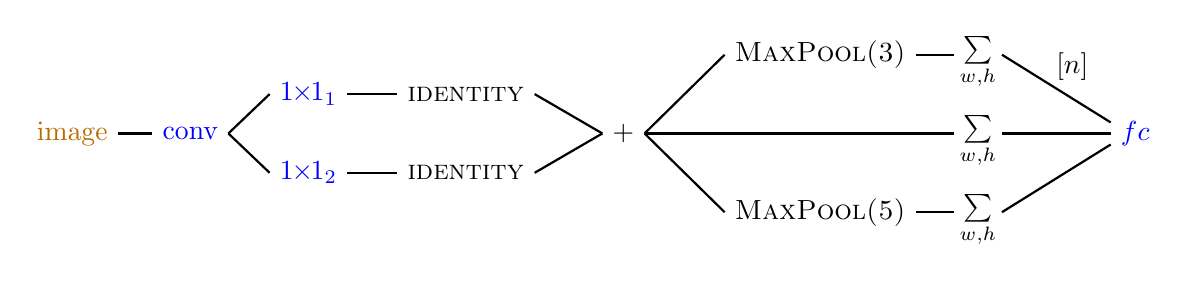
\begin{tikzpicture}
\begin{scope}[
  thick,decoration={
        markings,
        %mark=at position 0.5 with {\arrow{>}}
      }
    ]
\node[text={rgb:red,4;green,2;yellow,1}] (image) at (0,0) {image};
\node[text=blue] (conv) at (1.5, 0) {conv};
\draw[postaction={decorate}] (image.east) -- (conv.west);

\node[text=blue] (a11) at (3, -0.5) {$1\TMS1_2$};
\node[text=blue] (b11) at (3, 0.5) {$1\TMS1_1$};
\draw[postaction={decorate}] (conv.east) -- (a11.west);
\draw[postaction={decorate}] (conv.east) -- (b11.west);

\node (sm_3) at (5.0, -0.5) {\textsc{identity}};
\node (sm_4) at (5.0,  0.5) {\textsc{identity}};
\draw[postaction={decorate}] (a11.east) -- (sm_3.west);
\draw[postaction={decorate}] (b11.east) -- (sm_4.west);


\node (p_2) at (7,  0) {$+$};
\draw[postaction={decorate}] (sm_3.east) -- (p_2.west);
\draw[postaction={decorate}] (sm_4.east) -- (p_2.west);

\node (mp3) at (9.5, 1) {\textsc{MaxPool(3)}};
\node (mp5) at (9.5, -1) {\textsc{MaxPool(5)}};
\draw[postaction={decorate}] (p_2.east) -- (mp3.west);
\draw[postaction={decorate}] (p_2.east) -- (mp5.west);

\node (h_1) at (11.5,  0)  [label={[xshift=0.0cm, yshift=-0.7cm]$\sum\limits_{w,h}$}] {\ \ \ \ };
\node (h_2) at (11.5,  -1)  [label={[xshift=0.0cm, yshift=-0.7cm]$\sum\limits_{w,h}$}] {\ \ \ \ };
\node (h_3) at (11.5,  1)  [label={[xshift=0.0cm, yshift=-0.7cm]$\sum\limits_{w,h}$}] {\ \ \ \ };
%\node (h_1) at (11.5,  0) {$\sum\limits_{w,h}$};
%\node (h_2) at (11.5, -1) {$\sum\limits_{w,h}$};
%\node (h_3) at (11.5,  1) {$\sum\limits_{w,h}$};

\node (num) at (12.7,  0.85) {$[n]$};

\draw[postaction={decorate}] (p_2.east) -- (h_1.west);
\draw[postaction={decorate}] (mp3.east) -- (h_3.west);
\draw[postaction={decorate}] (mp5.east) -- (h_2.west);

\node[text=blue] (fc) at (13.5, 0) {$fc$};
\draw[postaction={decorate}] (h_1.east) -- (fc.west);
\draw[postaction={decorate}]  (h_2.east) -- ([yshift=-4pt] fc.west);
\draw[postaction={decorate}]  (h_3.east) -- ([yshift=4pt] fc.west);

%\path (a11) -- (b11) node [midway, sloped] {$\dots$};
%\path (mp3.south) -- (9.5, 0.10) node [midway, sloped] {$\dots$};

\end{scope}
\end{tikzpicture}
}
\caption{Model data-flow used for All-Pairs.}
\label{typenet_fig_sup}
\end{figure*}

\begin{table}[!htb]
  \centering%
    \begin{tabular}{ l l }
    parameter & value \\
    \hline
    $N_c$ & 4  \\
    $N_f$ & 4  \\
    $N_t$ & 2  \\
    $N_s$ & 3  \\
    $n$ & 64  \\
    \textsc{Ac} & \textsc{Elu}  \\
    \textsc{A} & \textsc{Identity}  \\
    \textsc{Spatial} & \{\textsc{Identity}, \textsc{MaxPool3x3}, \textsc{MaxPool5x5}\}  \\
    \textsc{Afc} & \textsc{Elu}  \\
    \end{tabular}
  \caption{Model level parameters for TypeNet as used to solve All-Pairs.}\label{global_config}
\end{table}

\noindent
For the activation, \textsc{A}$_i$, the most useful activations were found to be \textsc{Identity}, \textsc{Selu}, and
\textsc{SoftMax}.  \textsc{SoftMax} is in the feature, rather than spatial
dimension.  Via architecture search, \textsc{Identity} is the most generally useful activation, though \textsc{SoftMax} tended to reduce training times (probably because it forms a strong approximately-sparse bottleneck).  

The convolution block used \textsc{Elu} activation, no bias, batch norm (post-activation),
and padding to align the convolution filters with the image edges.  It's layer-wise characteristics are detailed below.  For larger images, a stride of 2 was used in \textsc{Conv}$_3$.
\begin{table}[!htb]
  \centering%
    \begin{tabular}{ l l }
    parameter & features, size, stride  \\
    \hline
    \textsc{Conv}$_1$ & 128, 3, 1  \\ 
    \textsc{Conv}$_2$ & 128, 5, 2  \\
    \textsc{Conv}$_3$ & 128, 5, 1  \\
    \textsc{Conv}$_4$ & 128, 3, 1  \\
    \end{tabular}
  \caption{Convolution block parameters for TypeNet as used to solve All-Pairs.}\label{detail_config_1}
\end{table}

\noindent
The fully-connected layers have input of size $m=N_s \TMS n$ and their configuration is detailed below:
\begin{table}[!htb]
  \centering%
    {\renewcommand{\arraystretch}{1.15}
    \begin{tabular}{ l l }
    parameter & value  \\
    \hline
    $fc_1$ & $m$-\textsc{Elu}-bnorm  \\
    $fc_2$ & $\floor*{\frac{m}{2}}$-\textsc{Elu}-bnorm  \\
    $fc_3$ & $\floor*{\frac{m}{4}}$-\textsc{Elu}-bnorm  \\
    $fc_4$ & $2$-\textsc{Identity}  \\
    \end{tabular}
    }
  \caption{Fully-connected parameters for TypeNet as used to solve All-Pairs.}\label{detail_config_2}
\end{table}

\subsection{TypeNet Architecture Search} \label{allpairsresult_sup}

The main hyper-parameters and architecture-variations explored are the
feature activation, number of branches ($k$), and number of features
($n$).  First, we explored the choice of activation with $n=64$ and
$k=2$.  All activation combinations drawn from the following options
were explored and the top results are presented in Figure
\ref{arch_search_fig} : \textsc{Elu} ($\mathsf{E}$), \textsc{Identity} ($\mathsf{I}$), \textsc{Relu} ($\mathsf{R}$), \textsc{Selu} ($\mathsf{Se}$),
\textsc{Sigmoid} ($\mathsf{S}$), \textsc{SoftMax} ($\mathsf{Sm}$), \textsc{SoftPlus} ($\mathsf{Sp}$), and \textsc{Tanh} ($\mathsf{T}$).
In each figure, architectures are labeled with $n$ when $n\neq64$, and the
above abbreviations of the $k$ activations are used.  If a ``$\dashw$'' is appended,
the architecture had a wider convolution receptive field (the stride of the
third \textbf{conv} layer was 2).
%\small
\begin{equation} \label{archnotation_sup:1}
%\mathtt{[n\#-] activation_1 [activation_2 ... activation_k]}.
\mathsf{[\ndash] Activation_1 [... Activation_k]}[\dashw].
\end{equation}
%\normalsize

All of the runs represented in Figure \ref{arch_search_fig} had
higher accuracy than any of the baselines.  The main conclusion from
these trials is that \textsc{SoftMax} and \textsc{Selu} are the most useful
activations.  We most frequently used \textsc{SoftMax} as the activation in
exploring the other hyper-parameters because of its low training
variance.

We studied how the number of branches, $k$, affects training; those
results are shown below with the number of training samples needed to
fully solve the 4-4 All-Pairs problem.  All trials reached 100\% accuracy,
save for one three-branch trial which got stuck at a test accuracy of
99.948\% after 30M training examples.  Based on the number of samples
needed to reach maximum test accuracy, we conclude that $k=2$ is best
for this problem.
\begin{center}
\begin{tabular}{ l l l }
branches ($k$) & accuracy  & training samples \\
\hline
 1 [$\times$9] & $1.0 \pm 0.0$                     & $57.1M \pm 3.8M$ \\
 2 [$\times$10] & $1.0 \pm 0.0$                   & $47.7M \pm 4.7M$    \\
 3 [$\times$20] & $1.0 \pm 10^{-4}$     & $49.4M \pm 8.9M$   \\
%  3 [$\times$20] & $0.99997 \pm 10^{-4}$     & $49.4M \pm 8.9M$   \\
\end{tabular}\label{branches}
\end{center}
The \textsc{SoftMax} activated network with two branches was found to train
faster for more features as summarized in the following table:  \\
\begin{center}
\begin{tabular}{ l l l }
features ($n$) & accuracy  & training samples \\
\hline
 48 [$\times$9] & $1.0 \pm 0.0$       & $57.0M \pm 8.9M$ \\
 64 [$\times$10] & $1.0 \pm 0.0$     & $47.7M \pm 4.7M$    \\
 96 [$\times$20] & $1.0 \pm 0.0$     & $40.5M \pm 7.7M$.   \\
\end{tabular} \\
\end{center}
All options consistently achieved 100\% test accuracy, so this trade-off
for the 4-4 problem can be made to optimize training time or inference
time.

\begin{figure*}[!htb]
\centering
\minipage{0.74\textwidth}
  \includegraphics[width=\linewidth]{images/arch_test_4_4}
\endminipage\hfill
\caption{4-4 All-Pairs for different activation functions, \textsc{A}$_i$.}
\label{arch_search_fig}
\end{figure*}

\subsection{More Details on the Harder All-Pairs Problems}

\begin{figure*}[!htb]
\minipage{0.23\textwidth}
  %\includegraphics[width=\linewidth]{images/missed_examples_77}
  %\includegraphics[width=\linewidth]{images/missed_examples_77_highlight}
  \includegraphics[width=\linewidth]{images/missed_examples_77_highlight_red}
  \endminipage\hfill
\minipage{0.74\textwidth}
  \includegraphics[width=\linewidth]{images/even_harder}
\endminipage\hfill
\caption{\emph{Left}: Examples of incorrect test samples from TypeNet $\mathsf{96{\text -}II{\text -}w}$ trained on 7-7 All-Pairs for 200M samples.  White symbols can be paired, leaving the red symbols unpaired.
  \emph{Right}: Test results of applying TypeNet to more difficult All-Pairs problems.  Wider \textbf{conv} receptive fields are notated with ``-$\mathsf{w}$'', see text for details. }
\label{missed_sup}
\end{figure*}

% ------------------------

The TypeNet approach cannot easily be made to solve every All-Pairs
problem; Figure \ref{missed_sup} shows results for the 5-5, 6-6, and 7-7 All-Pairs problem.
The \textsc{Identity} activation was the only activation to reach 100\% accuracy on the
5-5 and 6-6 problem, in 100\% (Fig\ref{missed_sup}-a) and 20\% (Fig\ref{missed_sup}-d) of trials respectively.  The \textsc{Selu} and \textsc{SoftMax} activation
were not successful on any of these problems in any trail within the 100M
training sample limit.

For these problems, the image size was increased
from $76\TMS76$ to $96\TMS96$ to make room for all the symbols.
This image size increase required decreasing the batch size from 600 to
400; all other training settings remained unchanged.  The large image size led us to expand the receptive field of the \textbf{conv} as notated with ``-$\mathsf{w}$'' and detailed in Section \ref{allpairsresult_sup}.  The most enlightening observations from these experiments are as follows:
\vspace{-4mm}
\begin{tightitemize}
\item The \textsc{Selu} activation (Fig\ref{missed_sup}-c) had lower accuracy
than expected from its effectiveness on the 4-4 problem.
\item On these harder problems, the \textsc{SoftMax} activation continued to
show lower variance across trials in both accuracy and training samples.
\item The $\mathsf{SmSm}$ model (Fig\ref{missed_sup}-b) consistently got stuck
at 94.6\% accuracy on the 5-5 problem, perhaps because the \textsc{SoftMax} activations are prone
to local minima.
\item The number of branches was increased to 3 and number of features to 128,
  independently and together, for the best case activations from smaller models.
  The $\mathsf{128{\text -}III}$ (Fig\ref{missed_sup}-f) model had the best test accuracy, but did worst than the simpler $\mathsf{II}$ model
  (Fig\ref{missed_sup}-e) even when trained to 200M training examples.
\item The 7-7 All-Pairs problem (Fig\ref{missed_sup}-g,h) is clearly
harder. The wider $\mathsf{96{\text -}II{\text -}w}$ (Fig\ref{missed_sup}-g) model was the best.
\item As shown in Figure \ref{missed_sup}-Left, the test samples missed by
one of the $\mathsf{96{\text -}II{\text -}w}$ models on the 7-7 problem are semantically similar: the
model incorrectly labels some samples as $true$ that have either an unpaired
\textbf{cross} and \textbf{3-star}, or an unpaired \textbf{theta} and \textbf{phi}.  For this model and trial, all of its errors fall into these two classes, though it correctly classifies some of those examples (achieving a 95\% accuracy when those two classes account for 9.5\% of the test set).  Different trials show different types of semantic errors.
\item Many variations, including mixtures of activations, more features, more branches, even wider \textbf{conv} receptive fields, and combinations of these choices, were tried to solve the 7-7 problem without success.  In the highest test accuracy observed (98\%), the misclassified images are still easy for a human to classify.
\end{tightitemize}

\subsection{Comparison to a Simple CNN}
\label{comptocnn}
\noindent
Are Lines 5 and 6 of Algorithm 1 generally useful, and do they improve the algorithm?
The table below compares (3 trials for each) the test accuracy and model size of TypeNet with a with a simple convolutional net (ConvNet) created by altering TypeNet as follows:
\begin{itemize}
\item Replace Lines 5 and 6 of Algorithm 1 with \textsc{Flatten} (passing the convolution output directly to the fully-connected layers).
\item As with larger All-Pairs images, use a stride of 2 in \textsc{Conv}$_3$.
\end{itemize}

%\begin{center}
%\begin{tabular}{ r | c c | c c  }
%              & \multicolumn{2}{c|}{ConvNet}                        & \multicolumn{2}{c}{TypeNet}  \\
%dataset  & accuracy & \# parameters & accuracy & \# parameters \\
%\hline
%MNIST               & 0.995167 $\pm$ 0.0004    & 1.39M & \textbf{0.9971 $\pm$ 0.0006} & \textbf{1M}  \\
%Fashion-MNIST & \textbf{0.938133 $\pm$ 0.0008}    & 1.39M & 0.9346 $\pm$ 0.0011 & \textbf{1M} \\
%CIFAR10           & 0.767500 $\pm$ 0.0028     & 1.39M & \textbf{0.8820 $\pm$ 0.0080} & \textbf{1M} \\
%4-4 All-Pairs      & 0.754600 $\pm$ 0.0000     & 3.45M & \textbf{1.0000 $\pm$ 0.0000} & \textbf{1M} \\
%\end{tabular}
%\end{center}

\begin{center}
\begin{tabular}{ r | c c | c c  }
              & \multicolumn{2}{c|}{ConvNet}                        & \multicolumn{2}{c}{TypeNet}  \\
dataset  & accuracy & \# parameters & accuracy & \# parameters \\
\hline
MNIST               & 0.9953 $\pm$ 0.0002    & 2M & \textbf{0.9971 $\pm$ 0.0006} & \textbf{1M}  \\
Fashion-MNIST & \textbf{0.9409 $\pm$ 0.0005}    & 2M & 0.9346 $\pm$ 0.0011 & \textbf{1M} \\
CIFAR10           & 0.7773 $\pm$ 0.0013     & 2.5M & \textbf{0.8820 $\pm$ 0.0080} & \textbf{1M} \\
4-4 All-Pairs      & 0.8080 $\pm$ 0.0925     & 9.9M & \textbf{1.0000 $\pm$ 0.0000} & \textbf{1M} \\
\end{tabular}
\end{center}

\noindent
From this comparison, TypeNet is seen to have fewer parameters and shows significant improvements in accuracy for the hardest two datasets (CIFAR10 and 4-4 All-Pairs).  The number of parameters in TypeNet is not dependent on the input size because of the spatial summation in Line 6 of the algorithm.  We anticipate the spatial, learned histogram of TypeNet to be a useful tool in the construction of other DNN architectures.

%\raggedbottom
%\vfill



\end{document}
